\documentclass{article}

\usepackage{amsmath, parskip, tikz}
\usetikzlibrary{automata}
\usetikzlibrary{positioning}
\usetikzlibrary{arrows}
\usepackage[margin=1.25in]{geometry}
\usepackage[shortlabels]{enumitem}

\renewcommand{\thesection}{\arabic{section}.}
\renewcommand{\thesubsection}{\alph{section}.}

\tikzset{
    node distance=2.5cm,
    every state/.append style={
        semithick,
        fill=gray!10
    },
    initial/.append style={
        initial text={},
        initial distance=0.5cm
    },
    accepting/.append style={
        double=gray!10,
        double distance=2pt,
        outer sep=1pt
    },
    every edge/.append style={
        draw,
        ->,>=stealth',
        auto,
        semithick
    }
}

\title{Homework 2: DFAs and NFAs}
\author{Will Griffin}

\begin{document}
    \maketitle

    \section{Divisibility Tests} 

    Define, for all $k > 0$,
    \begin{equation*}
        D_k = \{w \in \{0, \ldots, 9\}^* \mid w \text{ is the decimal representation of } k\}
    \end{equation*}
    where $\varepsilon$ is considered to represent the number 0. For example, the strings $\varepsilon$, \texttt{0}, \texttt{1234}, and \texttt{01234} all belong to $D_2$, but \texttt{99} and \texttt{099} do not.

    \begin{enumerate}[(\textasteriskcentered)]
        \item For any $k > 0$, the language $D_k$ is regular to the DFA $M = \left(Q, \Sigma, \delta, q_0, q_0\right)$ where
            \begin{itemize}
                \item $Q = \{q_0, \ldots, q_{k-1}\}$
                \item $\Sigma = \{0, \ldots, 9\}$
                \item $\delta (q_n, w \in \Sigma^*) = q_{(n \times 10 + w \pmod k)}$
            \end{itemize}
            For any $k > 0$, any whole number divided by $k$ has a remainder between $0$ and $k-1$. Therefore, the number of possible remainders for dividing a number by $k$ is equal to $k$, and thus the number of states for the DFA representing dividing a number by $k$ is equal to $k$. $Q$ is the set of all states of this DFA, where each state is numbered by the corresponding remainder ($Q = \{q_0, \ldots, q_{k-1}\}$). 

            By having each state correspond to a remainder, the DFA then stores the remainder of the number in the string $w \in \Sigma^*$ as each digit is processed. 

            Mathematically, the transition function $\delta$ operates as such on string $w \in \Sigma^*$: 
            \begin{enumerate}[(a)]
                \item Base Case ($w_1$):

                    The start state is $q_0$, so $r_{prev} = 0$. Therefore, $\delta (q_0, w_1) = q_{(0 \times 10 + w_1 \pmod k)} = q_{(w_1 \bmod k)}$

                \item Recursive Case ($w_i$, $0 < i \le |w|$):

                    The remainder of a number can be found through calculating the remainder of its digits one by one. If $N$ is the string of already read digits, and $d$ is the next digit, $N_{new} = N \times 10 + d$. Taking the modulus with respect to k, we obtain the remainder of $N_{new}$ calculated from the remainder of $N$:
                    
                    \begin{align*}
                        N_{new} \bmod k &= (N \times 10 + d) \bmod k \\
                        r_{new} &= (((N \bmod k)(10 \bmod k) \bmod k) + (d \bmod k)) \bmod k \footnotemark\\
                        r_{new} &= ((R \times (10 \bmod k) \bmod k) + (d \bmod k)) \bmod k \\
                        r_{new} &= (R \times 10 + d) \bmod k
                    \end{align*}

                    We can apply this to the transition function $\delta$, such that for a DFA at current state $q_j$, $j \in [0, k-1]$, processing symbol $w_i \in w$, $\delta (q_j, w_i) = q_{((j \times 10 + w_i) \bmod k)}$.

            \end{enumerate}

    \end{enumerate}

    \section{Nondeterminism}
        \begin{enumerate}[(a)]
            \item The computation of \texttt{1110100} on $N_2$.

                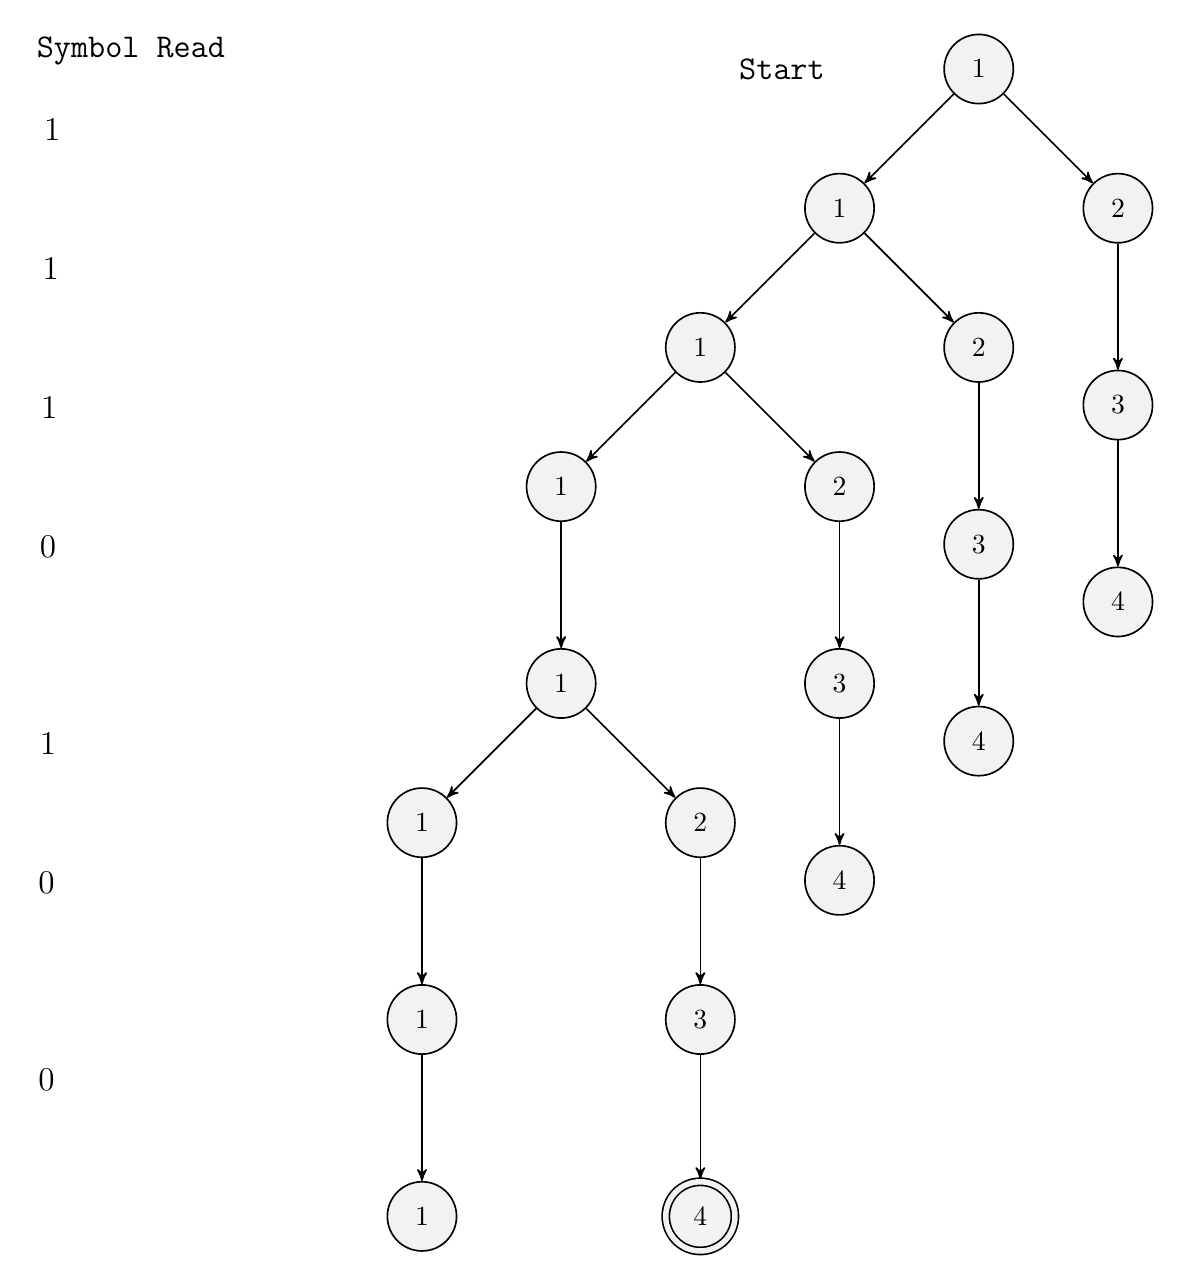
\begin{tikzpicture}[label node/.style={font=\ttfamily\large, anchor=east}]
                    \node[state] (01) {$1$};
                    \node[label node, left of = 01] (lstart) {\texttt{Start}};
                    \node[label node, below left of = 01, xshift=-10cm, yshift=1cm] (l1) {$1$};
                    \node[label node, above of = l1, yshift=-1.5cm, xshift=1cm] (lsr) {\texttt{Symbol Read}};
                    \node[state, below left of = 01] (11) {$1$};
                    \node[state, below right of = 01] (12) {$2$};
                    \node[label node, below left of = 11, xshift=-8.25cm, yshift=1cm] (l2) {$1$};
                    \node[state, below left of = 11] (21) {$1$};
                    \node[state, below right of = 11] (22) {$2$};
                    \node[state, below of = 12] (23) {$3$};
                    \node[label node, below left of = 21, xshift=-6.5cm, yshift=1cm] (l3) {$1$};
                    \node[state, below left of = 21] (31) {$1$};
                    \node[state, below right of = 21] (32) {$2$};
                    \node[state, below of = 22] (33) {$3$};
                    \node[state, below of = 23] (34) {$4$};
                    \node[label node, below left of = 31, xshift=-4.75cm, yshift=1cm] (l4) {$0$};
                    \node[state, below of = 31] (41) {$1$};
                    \node[state, below of = 32] (43) {$3$};
                    \node[state, below of = 33] (44) {$4$};
                    \node[label node, below left of = 41, xshift=-4.75cm, yshift=1cm] (l5) {$1$};
                    \node[state, below left of = 41] (51) {$1$};
                    \node[state, below right of = 41] (52) {$2$};
                    \node[state, below of = 43] (54) {$4$};
                    \node[label node, below left of = 51, xshift=-3cm, yshift=1cm] (l6) {$0$};
                    \node[state, below of = 51] (61) {$1$};
                    \node[state, below of = 52] (63) {$3$};
                    \node[label node, below left of = 61, xshift=-3cm, yshift=1cm] (l7) {$0$};
                    \node[state, below of = 61] (71) {$1$};
                    \node[state, below of = 63, accepting] (74) {$4$};

                    \draw (01) edge node {} (11)
                        edge node {} (12);
                    \draw (11) edge node {} (21)
                        edge node {} (22);
                    \draw (12) edge node {} (23);
                    \draw (21) edge node {} (31)
                        edge node {} (32);
                    \draw (22) edge node {} (33);
                    \draw (23) edge node {} (34);
                    \draw (31) edge node {} (41);
                    \draw (32) edge node {} (43);
                    \draw (33) edge node {} (44);
                    \draw (41) edge node {} (51)
                        edge node {} (52);
                    \draw (43) edge node {} (54);
                    \draw (51) edge node {} (61);
                    \draw (52) edge node {} (63);
                    \draw (61) edge node {} (71);
                    \draw (63) edge node {} (74);
                \end{tikzpicture}

            \item The DFA $M$ of the NFA $N_2$

                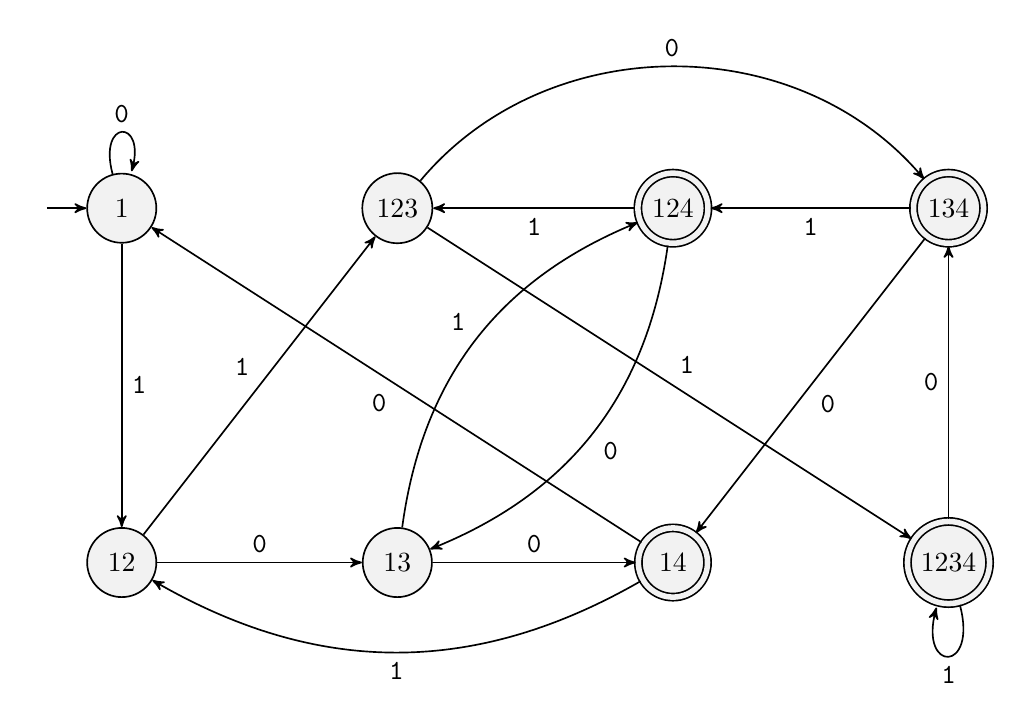
\begin{tikzpicture}
                    \node[state, initial] (1) {$1$};
                    \node[state, below of = 1, yshift=-2cm] (12) {$12$};
                    \node[state, right of = 12, xshift=1cm] (13) {$13$};
                    \node[state, right of = 13, xshift = 1cm, accepting] (14) {$14$};
                    \node[state, right of = 14, xshift = 1cm, accepting] (1234) {$1234$};
                    \node[state, right of = 1, xshift = 1cm] (123) {$123$};
                    \node[state, right of = 123, xshift = 1cm, accepting] (124) {$124$};
                    \node[state, right of = 124, xshift = 1cm, accepting] (134) {$134$};

                    \draw (1) edge[loop above] node {\texttt{0}} (1)
                        edge node {\texttt{1}} (12);
                    \draw (12) edge node {\texttt{0}} (13)
                        edge node {\texttt{1}} (123);
                    \draw (13) edge node {\texttt{0}} (14)
                        edge[bend left] node {\texttt{1}} (124);
                    \draw (14) edge node {\texttt{0}} (1)
                        edge[bend left] node {\texttt{1}} (12);
                    \draw (1234) edge node {\texttt{0}} (134)
                        edge[loop below] node {\texttt{1}} (1234);
                    \draw (123) edge[bend left=50] node {\texttt{0}} (134)
                        edge node {\texttt{1}} (1234);
                    \draw (124) edge[bend left] node {\texttt{0}} (13)
                        edge node {\texttt{1}} (123);
                    \draw (134) edge node {\texttt{0}} (14)
                        edge node {\texttt{1}} (124);

                \end{tikzpicture}

            \item The order \texttt{1110100} goes through $M$ is:
                \begin{itemize}
                    \item 1
                    \item 12
                    \item 123
                    \item 1234
                    \item 134
                    \item 124
                    \item 134
                    \item 14
                \end{itemize}

            \item The states in the DFA of Figure 1.31 have subscripts containing the last three digits read. It starts out assuming the last three digits read were \texttt{0}s, essentially a cleared input stream. As \texttt{1}s are read, they are input in the last digit and shifted left as more digits are read. It is also easier to obviously see success states; each state with notation $q_{1xx}$ will be a success state as it has a \texttt{1} in the third to last position.

            
        \end{enumerate}

    \section{Procrustean Closure Properties}

        \begin{enumerate}[(a)]
            \item Prove that for any regular language $L$, STRETCH($L$) is also regular.

                If $L$ is a regular language, there must be some DFA $M$ that recognizes it. Let that DFA $M = (Q, \Sigma, \delta, s, F)$.
                
                To prove STRETCH($L$) is also regular, let another DFA $M' = (Q', \Sigma, \delta', s', F')$ exist that recognizses STRETCH($L$).

                Since every symbol in $L$ is doubled when STRETCH($L$) is applied, we need to add a waiting state for every character in $\Sigma$. We also need to add a dead state so that when in any waiting state, if the succeeding character is different, the DFA moves to a dead state with no motion to success. Therefore, $Q' = Q \cup \{q_{\texttt{wait}, a} | q \in Q, a \in \Sigma\} \cup \{\texttt{DEAD}\}$.

                The transition function $\delta'$ will have three operations for any $q \in Q; a, b \in \Sigma, a \ne b$:
                \begin{itemize}
                    \item $\delta'(q, a) = q_{\texttt{wait}, a}$
                    \item $\delta'(q_{\texttt{wait}, a}, a) = \delta(q, a)$
                    \item $\delta'(q_{\texttt{wait}, a}, b) = \texttt{DEAD}$
                \end{itemize}

                Since both $M$ and $M'$ are at the very beginning of their computation before reading characters, therefore $s' = s$.

                Since $L$ is regular to $M$ and STRETCH($L$) is regular to $M'$, and $\delta'$ after passing a \texttt{wait} state is the result of the original transition function $\delta$, clearly $F' = F$.

                Since we have constructed a DFA $M' = (Q', \Sigma, \delta', s', F')$ that accepts language STRETCH($L$) from a DFA $M$ that accepts language $L$, for any regular language $L$, STRETCH($L$) is also regular.

            \item Prove that for any regular language $L$, CHOP($L$) is also regular.

                If $L$ is a regular language, there must be some DFA $M$ that recognizes. Let that DFA $M = (Q, \Sigma, \delta, s, F)$.

                To prove CHOP($L$) is a regular language, let a DFA $M' = (Q', \Sigma, \delta', s', F')$ exist that recognizes CHOP($L$).

                Since the CHOP($L$) operation removes the first symbol in the string, let the start state's transitions be defined as $\delta'(s', w_2) = \delta(\delta(s, w_1), w_2)$ where $w \in L, w = w_1 w_2 \ldots w_{n-1} w_n$.
                
                Since the CHOP($L$) operation also removes the last symbol in the string, let the state of accept states $F'$ be defined as $F' = \{q \mid \delta(q, a) = q_f, a \in \Sigma, q_f \in F\} \cup \{s' \mid \varepsilon \in$ CHOP($L$)$\}$.

                Let $Q' = (Q \setminus (\{s\} \cup \{q \mid \delta(s, w_1) = q, w \in L, w = w_1 w_2 \ldots w_n\} \cup F)) \cup \{s'\} \cup F'$.

                Since we have constructed a DFA $M'$ that accepts language CHOP($L$), for any regular language $L$, CHOP($L$) is also regular.
                 

        \end{enumerate}

    \section{References}

    \begin{enumerate}[(1)]
        \item "Modulo/Properties." \textit{Wikipedia}, Wikimedia Foundation, 21 Jan. 2026, \\ \texttt{https://en.wikipedia.org/wiki/Modulo\#Properties\_(identities)}.
    \end{enumerate}
    
\end{document}
